\subsection{Metamodelos}

\begin{figure}[H]
\centering
\begin{minipage}{.4\textwidth}
  \centering
  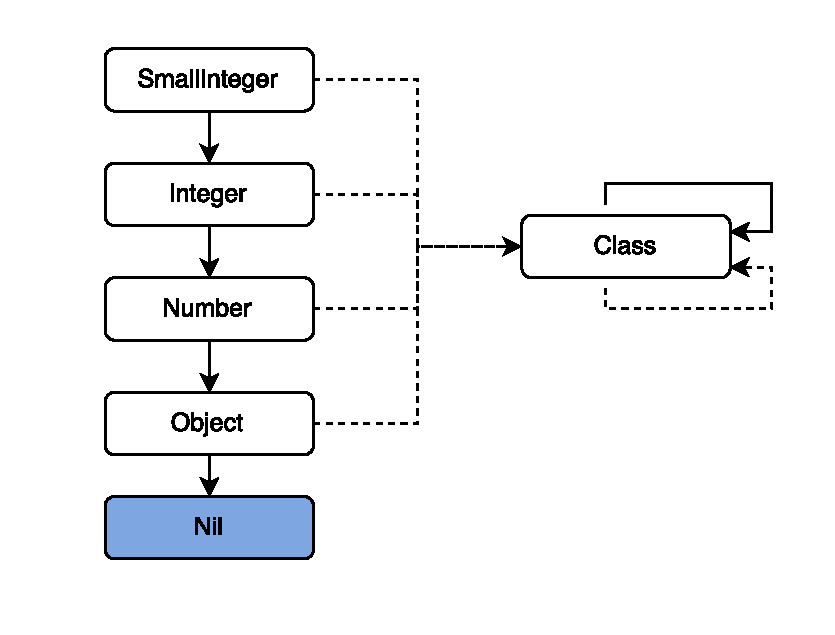
\includegraphics[width=\linewidth]{images/metamodelo_smalltalk_basico.pdf}
  \caption{Metamodelo B\'asico}
  \label{fig:metamodelo_basico}
\end{minipage}%
\begin{minipage}{.6\textwidth}
  \centering
  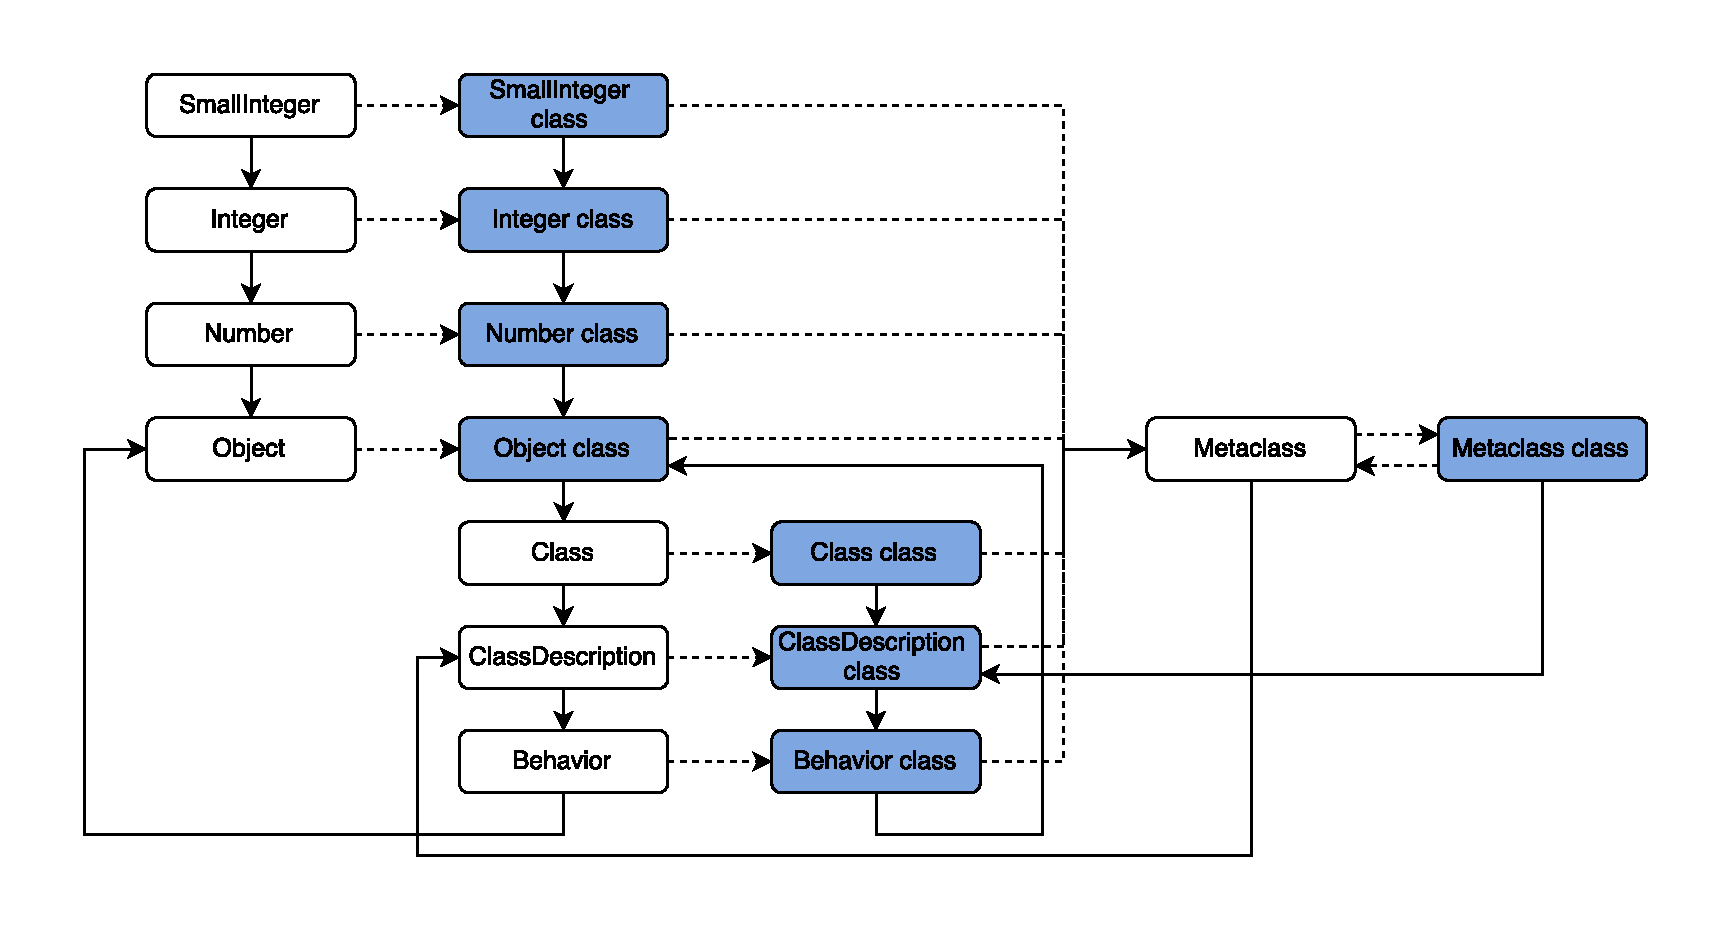
\includegraphics[width=1.2\linewidth]{images/metamodelo_smalltalk_80.pdf}
  \caption{Metamodelo SmallTalk80}
  \label{fig:metamodelo_st80}
\end{minipage}
\label{fig:test}
\end{figure}

Notemos que en el modelo b\'asico, todos los objetos son instancias de una sola clase. Todos comparten el mismo protocolo, ie, contestan los mismos mensajes. Esto es un problema, porque no podemos hacer mensajes exclusivos para distintos objetos. El objeto \code{Date} puede contestar el mensaje \code{today}, que un numero no puede. 

Por eso surge el segundo metamodelo. Para implementar distintos protocolos a cada clase y que cada objeto tenga su comportamiento. 

\begin{figure}[H]
  \begin{center}
  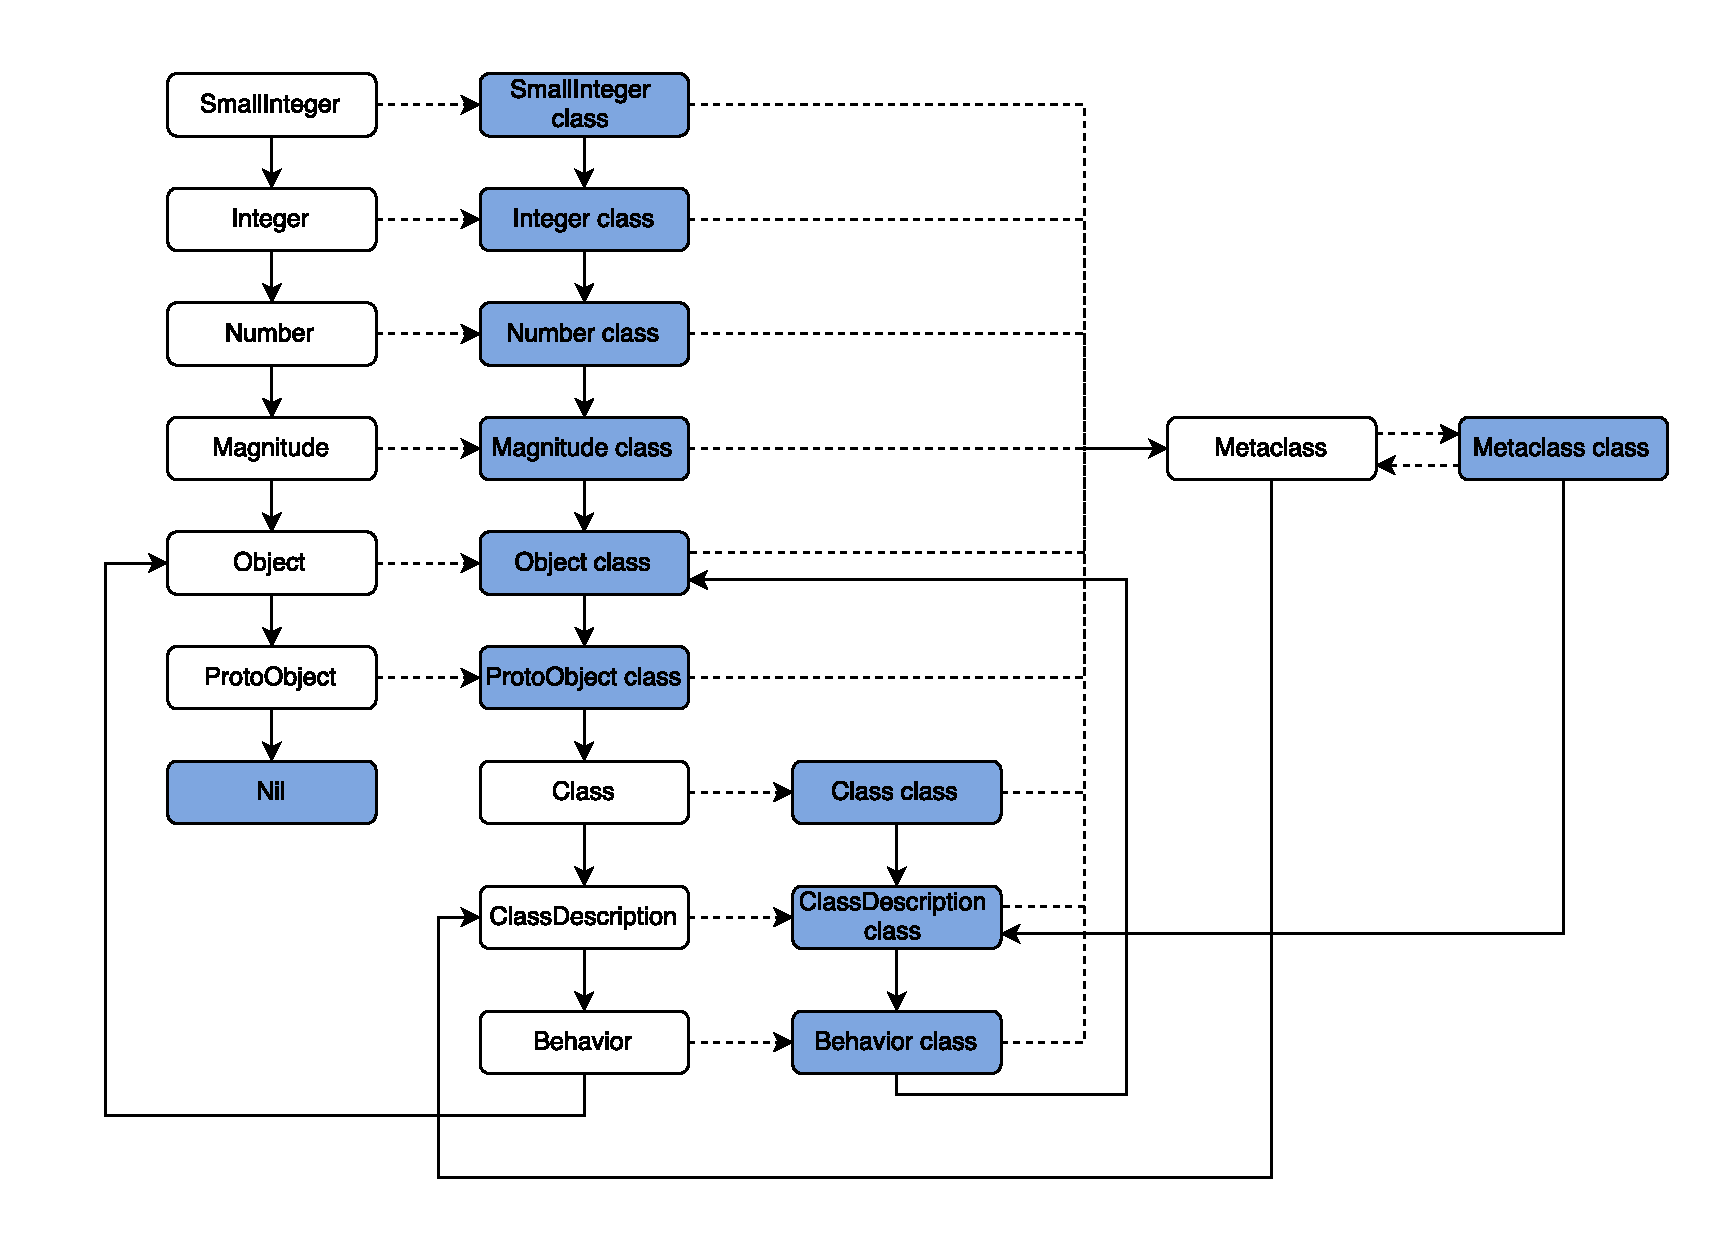
\includegraphics[height=300px]{images/metamodelo_smalltalk.pdf}
  \end{center}
  \caption{Metamodelo de Pharo4.0}
  \label{fig:metamodelo_pharo}
\end{figure}

\begin{figure}[H]
\centering
\begin{minipage}{.5\textwidth}
  \centering
  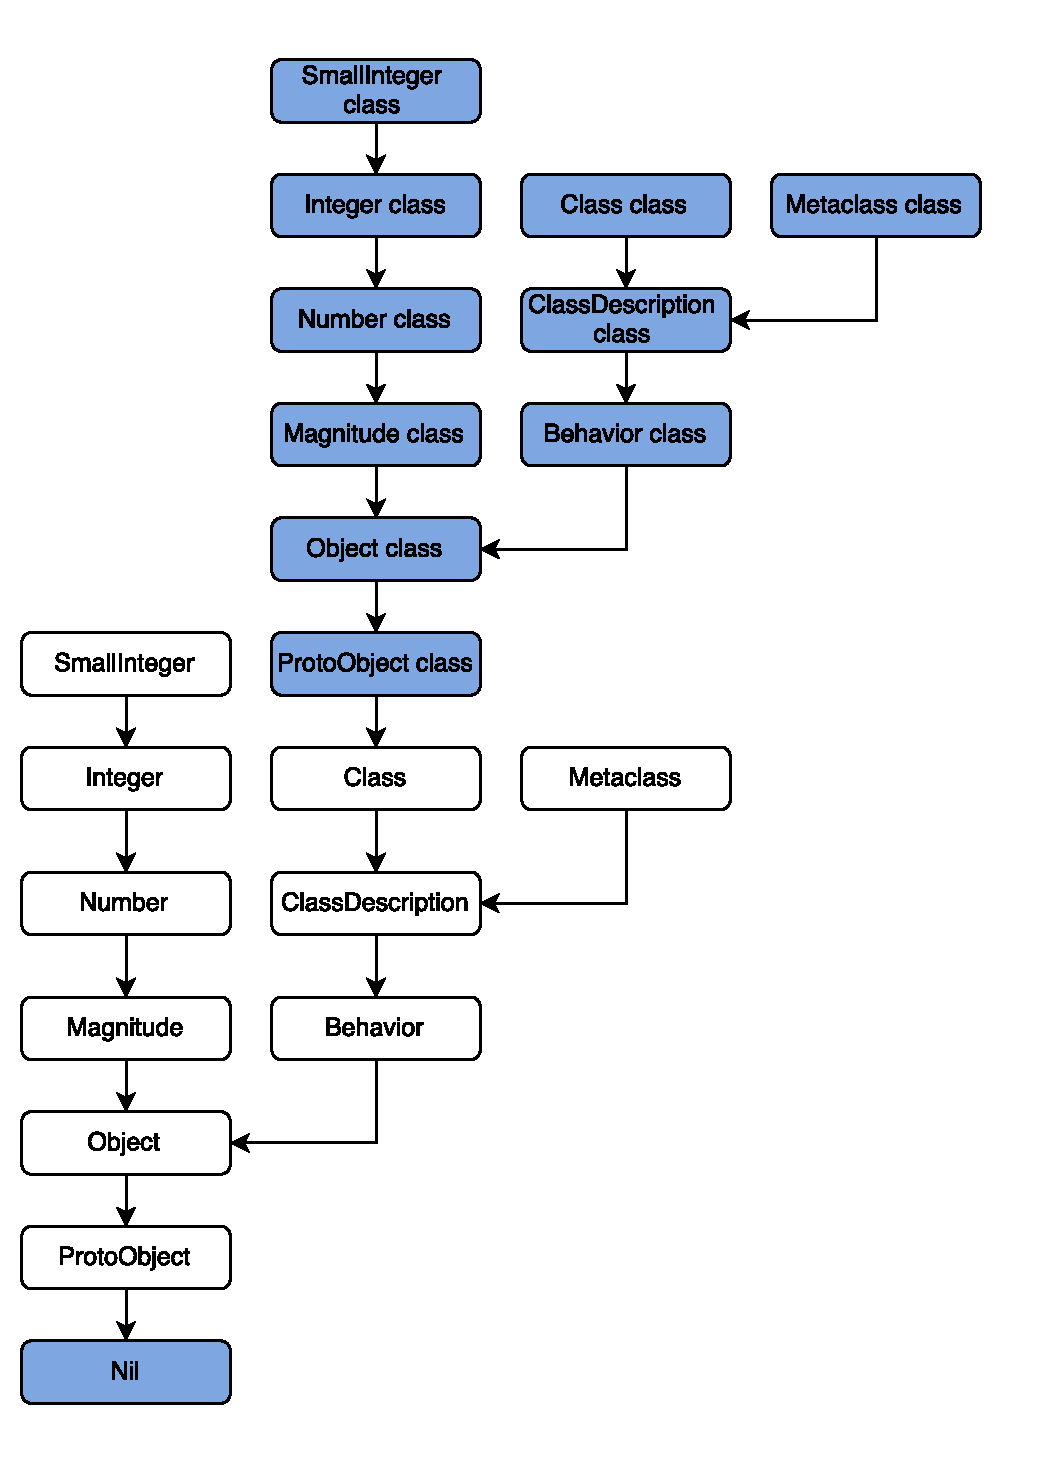
\includegraphics[width=\linewidth]{images/metamodelo_superclases.pdf}
  \caption{Grafo de Subclasificaciones}
  \label{fig:sub1}
\end{minipage}%
\begin{minipage}{.5\textwidth}
  \centering
  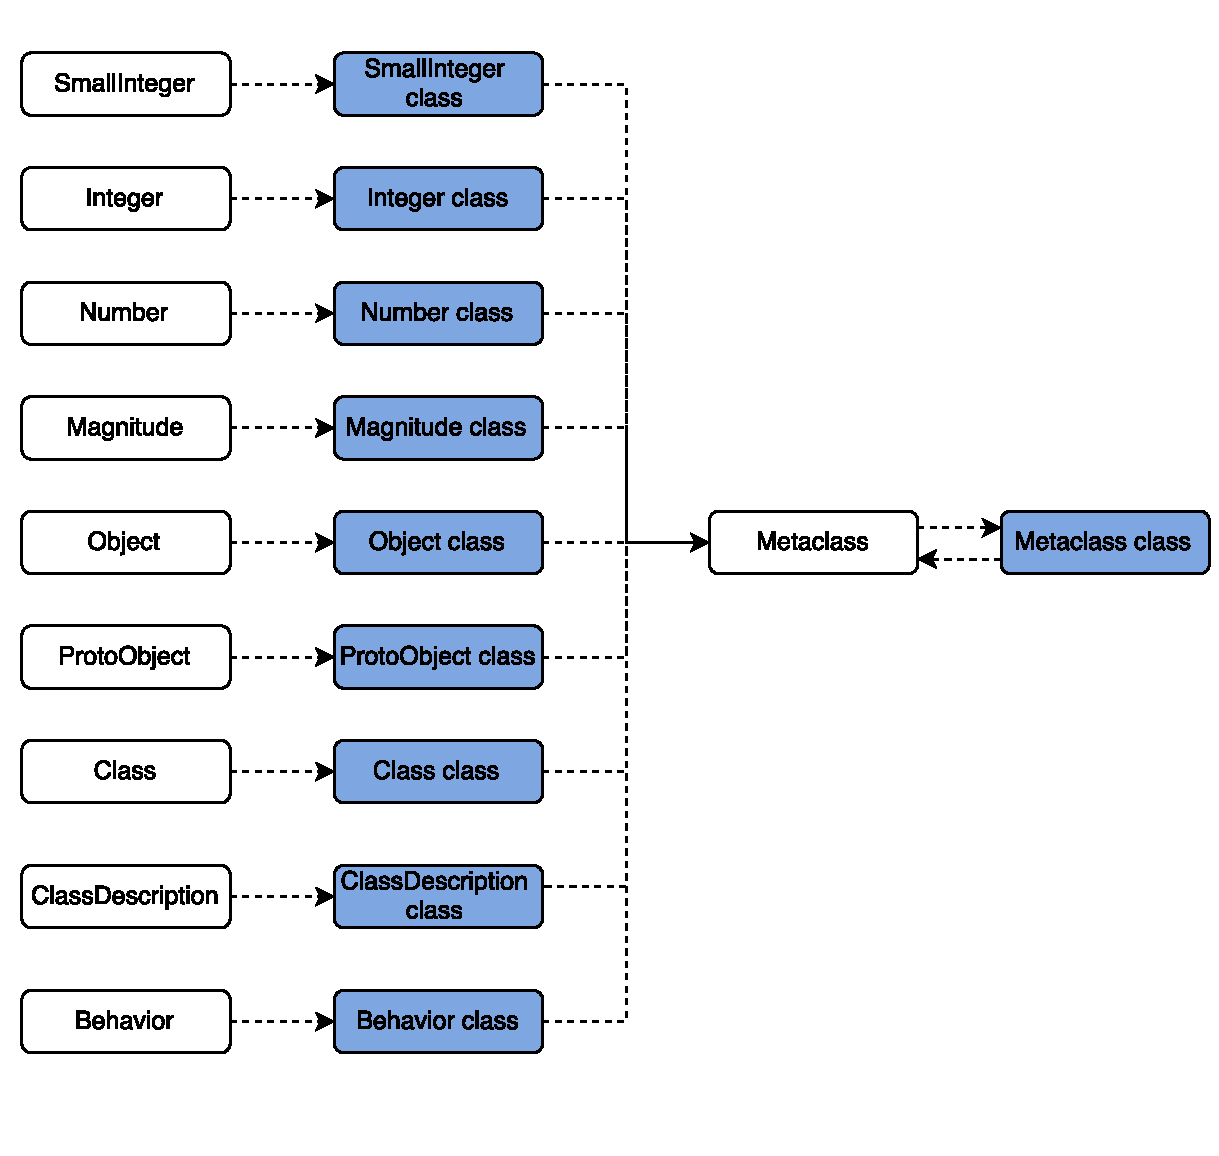
\includegraphics[width=1.2\linewidth]{images/metamodelo_instancia_de.pdf}
  \caption{Grafo ``Instancia de''}
  \label{fig:sub2}
\end{minipage}
\caption{Metamodelo de Pharo4.0}
\label{fig:test}
\end{figure}

\underline{Referencias}: Linea punteada significa ``Instancia de'', y Linea lisa ``Hereda de''.

\begin{enumerate}
 \item Los objetos en azul (?`las metaclases?), solo tienen una instancia. No contestan al mensaje \code{new}. ?`Qui\'en hace la alocaci\'on por primera vez? 
 
 Si a una metaclase se le agregan variables de instancia que inicializo en su m\'etodo \code{initialize} pero luego las modifico, debo reinicializar la metaclase para que se apliquen los cambios a las variables. No es como el caso de las variables de instancia de una clase. 
 
 \item Cuando se env\'ia \code{new} a cualquier objeto, el que aloca la memoria es \code{Behavior>>basicNew}. 
  \begin{enumerate}
    \item Siempre que se implementa \code{new} en una subclase, hay que llamar primero a \code{super new} para hacer la alocaci\'on. 
    
    \item Si es \code{Behavior} quien implementa la alocaci\'on, ?`qui\'en lo hace para \code{Object} y los que subclasifican de \'el? 
    
    Cuando un objeto recibe el mensaje \code{new}, busca su implementaci\'on en el protocolo de su clase, si este no la tiene lo busca en su padre, y as\'i sucesivamente hasta eventualmente llegar a \code{Behavior} que s\'i lo tiene. 
    
    \item \code{ProtoObject new} tira el siguiente error y se rompe todo: 

	\begin{verbatim}
	*** System error handling failed ***
	Original error: MessageNotUnderstood: ProtoObject>>inspect.
	\end{verbatim}

	?`Tiene algo que ver? No, simplemente que \code{ProtoObject} no est\'a preparado para ser debugeado, por eso es que no se puede mensajear dentro de Pharo. Esta clase surgi\'o en Pharo para hacer cosas como inspectores y m\'aquinas virtuales. 
    
  \end{enumerate}

 \item Enviarle la colaboraci\'on \code{superclass} a un objeto me devuelve lo que apunta la flecha lisa. Ej: 
\begin{verbatim}
SmallInteger superclass
>> Integer
Metaclass superclass
>> ClassDescription
\end{verbatim}

 \item Enviarle la colaboraci\'on \code{class} a un objeto me devuelve lo que apunta la flecha punteada. Ej: 
\begin{verbatim}
SmallInteger class
>> Smallinteger class
Integer class class
>> Metaclass
\end{verbatim}
  
 \item Enviar la colaboraci\'on \code{Metaclass new new} hace colgar Pharo. ?`Por qu\'e? ?`Es el \'unico objeto con el que pasa eso? 

 Casos border que est\'an mal implementados en Pharo. 
\end{enumerate}